%% abtex2-modelo-projeto-pesquisa.tex, v-1.7.1 laurocesar
%% Copyright 2012-2013 by abnTeX2 group at http://abntex2.googlecode.com/ 
%%
%% This work may be distributed and/or modified under the
%% conditions of the LaTeX Project Public License, either version 1.3
%% of this license or (at your option) any later version.
%% The latest version of this license is in
%%   http://www.latex-project.org/lppl.txt
%% and version 1.3 or later is part of all distributions of LaTeX
%% version 2005/12/01 or later.
%%
%% This work has the LPPL maintenance status `maintained'.
%% 
%% The Current Maintainer of this work is the abnTeX2 team, led
%% by Lauro César Araujo. Further information are available on 
%% http://abntex2.googlecode.com/
%%
%% This work consists of the files abntex2-modelo-projeto-pesquisa.tex
%% and abntex2-modelo-references.bib
%%

% ------------------------------------------------------------------------
% ------------------------------------------------------------------------
% abnTeX2: Modelo de Projeto de pesquisa em conformidade com 
% ABNT NBR 15287:2011 Informação e documentação - Projeto de pesquisa -
% Apresentação 
% ------------------------------------------------------------------------ 
% ------------------------------------------------------------------------

\documentclass[
	% -- opções da classe memoir --
	12pt,				% tamanho da fonte
	openright,			% capítulos começam em pág ímpar (insere página vazia caso preciso)
	twoside,			% para impressão em verso e anverso. Oposto a oneside
	a4paper,			% tamanho do papel. 
	% -- opções da classe abntex2 --
	%chapter=TITLE,		% títulos de capítulos convertidos em letras maiúsculas
	%section=TITLE,		% títulos de seções convertidos em letras maiúsculas
	%subsection=TITLE,	% títulos de subseções convertidos em letras maiúsculas
	%subsubsection=TITLE,% títulos de subsubseções convertidos em letras maiúsculas
	% -- opções do pacote babel --
	english,			% idioma adicional para hifenização
	french,				% idioma adicional para hifenização
	spanish,			% idioma adicional para hifenização
	brazil,				% o último idioma é o principal do documento
	]{abntex2}

% ---
% PACOTES
% ---

% ---
% Pacotes fundamentais 
% ---
\usepackage{cmap}				% Mapear caracteres especiais no PDF
\usepackage{lmodern}			% Usa a fonte Latin Modern
\usepackage[T1]{fontenc}		% Selecao de codigos de fonte.
\usepackage[utf8]{inputenc}		% Codificacao do documento (conversão automática dos acentos)
\usepackage{indentfirst}		% Indenta o primeiro parágrafo de cada seção.
\usepackage{color}				% Controle das cores
\usepackage{graphicx}			% Inclusão de gráficos
% ---

% ---
% Pacotes adicionais, usados apenas no âmbito do Modelo Canônico do abnteX2
% ---
\usepackage{lipsum}				% para geração de dummy text
% ---

% ---
% Pacotes de citações
% ---
\usepackage[brazilian,hyperpageref]{backref}	 % Paginas com as citações na bibl
\usepackage[alf]{abntex2cite}	% Citações padrão ABNT
\graphicspath{ {images/} }

% --- 
% CONFIGURAÇÕES DE PACOTES
% --- 

% ---
% Configurações do pacote backref
% Usado sem a opção hyperpageref de backref
\renewcommand{\backrefpagesname}{Citado na(s) página(s):~}
% Texto padrão antes do número das páginas
\renewcommand{\backref}{}
% Define os textos da citação
\renewcommand*{\backrefalt}[4]{
	\ifcase #1 %
		Nenhuma citação no texto.%
	\or
		Citado na página #2.%
	\else
		Citado #1 vezes nas páginas #2.%
	\fi}%
% ---

% ---
% Informações de dados para CAPA e FOLHA DE ROSTO
% ---
\titulo{Título: Uma Abordagem para Estimativa de Dívida Técnica Arquitetural
por meio de Indicadores de Degradação Extraídos a partir de Repositórios
de Software. }
\autor{Candidato: Armando Soares Sousa }
\local{Brasil}
\data{2017, v-1.0}
\instituicao{%
  Universidade Federal do Ceará - UFC
  \par
  Mestrado e Doutorado em Ciência da Computação - UFC
  \par
  Programa de Pós-Graduação em Ciência da Computação}
\tipotrabalho{Tese (Doutorado)}
% O preambulo deve conter o tipo do trabalho, o objetivo, 
% o nome da instituição e a área de concentração 
\preambulo{Pré-projeto de pesquisa para seleção de Doutorado do Programa de Pós-Graduação em Ciência da Computação da UFC \LaTeX.}
% ---

% ---
% Configurações de aparência do PDF final

% alterando o aspecto da cor azul
\definecolor{blue}{RGB}{41,5,195}

% informações do PDF
\makeatletter
\hypersetup{
     	%pagebackref=true,
		pdftitle={\@title}, 
		pdfauthor={\@author},
    	pdfsubject={\imprimirpreambulo},
	    pdfcreator={LaTeX with abnTeX2},
		pdfkeywords={abnt}{latex}{abntex}{abntex2}{projeto de pesquisa}, 
		colorlinks=true,       		% false: boxed links; true: colored links
    	linkcolor=blue,          	% color of internal links
    	citecolor=blue,        		% color of links to bibliography
    	filecolor=magenta,      		% color of file links
		urlcolor=blue,
		bookmarksdepth=4
}
\makeatother
% --- 

% --- 
% Espaçamentos entre linhas e parágrafos 
% --- 

% O tamanho do parágrafo é dado por:
\setlength{\parindent}{1.3cm}

% Controle do espaçamento entre um parágrafo e outro:
\setlength{\parskip}{0.2cm}  % tente também \onelineskip

% ---
% compila o indice
% ---
\makeindex
% ---

% ----
% Início do documento
% ----
\begin{document}

% Retira espaço extra obsoleto entre as frases.
\frenchspacing 

% ----------------------------------------------------------
% ELEMENTOS PRÉ-TEXTUAIS
% ----------------------------------------------------------
% \pretextual

% ---
% Capa
% ---
\imprimircapa
% ---

% ---
% Folha de rosto
% ---
\imprimirfolhaderosto
% ---

% ---
% NOTA DA ABNT NBR 15287:2011, p. 4:
%  ``Se exigido pela entidade, apresentar os dados curriculares do autor em
%     folha ou página distinta após a folha de rosto.''
% ---

% ---
% inserir lista de ilustrações
% ---
\pdfbookmark[0]{\listfigurename}{lof}
\listoffigures*
\cleardoublepage
% ---

% ---
% inserir lista de tabelas
% ---
\pdfbookmark[0]{\listtablename}{lot}
\listoftables*
\cleardoublepage
% ---

% ---
% inserir lista de abreviaturas e siglas
% ---
\begin{siglas}
  \item[Fig.] Area of the $i^{th}$ component
  \item[456] Isto é um número
  \item[123] Isto é outro número
  \item[lauro cesar] este é o meu nome
\end{siglas}
% ---

% ---
% inserir lista de símbolos
% ---
\begin{simbolos}
  \item[$ \Gamma $] Letra grega Gama
  \item[$ \Lambda $] Lambda
  \item[$ \zeta $] Letra grega minúscula zeta
  \item[$ \in $] Pertence
\end{simbolos}
% ---

% ---
% inserir o sumario
% ---
\pdfbookmark[0]{\contentsname}{toc}
\tableofcontents*
\cleardoublepage
% ---


% ----------------------------------------------------------
% ELEMENTOS TEXTUAIS
% ----------------------------------------------------------
\textual

% ----------------------------------------------------------
% Introdução
% ----------------------------------------------------------
\chapter*[Resumo]{Resumo}
\addcontentsline{toc}{chapter}{Resumo}

\emph{Título do Projeto:} Uma Abordagem para Estimativa de Dívida
Técnica Arquitetural por meio de Indicadores de Degradação Extraídos
a partir de Repositórios de Software. 

\emph{Descrição Resumida:} Na medida que os sistemas de software ficam
mais complexos é preciso definir uma arquitetura de referência que
permita descrever os elementos, os relacionamentos entre os elementos,
seus comportamentos bem como propor uma estrutura base que permita
a construção, evolução e manutenção do software de forma organizada.
Entretanto, nem sempre a equipe de desenvolvimento segue de forma
rigorosa as orientações da arquitetura de software proposta. Com isso,
pode surgir uma degradação arquitetural no sistema ou parte dele.
A degradação arquitetural tem duas perspectivas: (i) erosão - violação
de regras; e (ii) desvio - que está relacionado com anomalias de código
fonte. Além disso, na medida que o tempo passa, existe um processo
onde o time de desenvolvimento tende a desviar de padrões adotados,
deixar de implementar ou omitir elementos importantes de projeto de
software como requisitos, design, testes, builds, releases entre outros,
o que pode configurar um acúmulo de dívida técnica que com o passar
do tempo pode onerar os gastos (tempo, recursos humanos e recursos
financeiros envolvidos no projeto de software) referentes a manutenção
e evolução do software. Este trabalho tem como objetivo fazer uma
análise da evolução do código registrado em repositórios de software
- através de técnicas de mineração de dados em repositórios de software
- comparando com as regras arquiteturais originais, anomalias de código
(bad smells), definir índices e indicadores para estimar a dívida
técnica arquitetural e com isso mostrar para a equipe de desenvolvimento
os locais ou áreas de degradação arquitetural de software que mais impactam no pagamento desta dívida técnica.

\emph{Palavras chaves:} Arquitetura de Software, Degradação Arquitetural
de Software, Dívida Técnica, Mineração de Repositório de Código.

\chapter{Introdução}
\index{Introdução}

A aplicação do conceito de arquitetura de software vem crescendo dentro
do contexto de engenharia de software desde dos anos 90. Visto que, os sistemas atuais vem se tornando muito mais complexos e com isso, a arquitetura de software é considerada um ponto central em projetos complexos de sistemas de larga escala. A aplicação e o uso de um bom projeto arquitetural de software pode trazer grandes benefícios para a equipe de desenvolvimento. Principalmente no que se refere a manutenção e evolução do software tanto em correções e/ou debug de erros quanto na inserção de novas funcionalidades no sistema sem quebrar a estrutura do mesmo. \citeonline{series/utcs/OquendoLB16}

Desde 2011 temos uma definição formal de arquitetura de software dada
pela ISO/IEC Standard 42010 \textquotedblleft System and Software
Engineering - Architecture description\textquotedbl{} como \textquotedblleft As
propriedades fundamentais de um sistema concretizadas em seus elementos,
relacionamentos, nos princípios de design e evolução\textquotedblright \citeonline{iso42010} 

A degradação arquitetural acontece quando na medida que o sistema
é implementado existe um desvio de implementação em relação a arquitetura original. Quando isso acontece pode haver uma quebra
na qualidade do sistema e com isso pode vir a dificultar a manutenção
, podendo surgir falhas ou inconsistências durante a evolução
do sistema. A degradação arquitetural pode ser classificada em duas
perspectivas: (i) erosão arquitetural - relacionada a alterações da
arquitetura descritiva que podem levar a violações de restrições de
design entre os componentes do sistema e (ii) desvio - relacionados
a alterações que violam restrições na arquitetura prescritiva, por
exemplo: violações referentes a modularidade (acoplamento e coesão). 

Segundo Lehman (1996) \textquotedblleft Na medida que um programa
é continuamente alterado, sua complexidade, reflete em uma deteriorização
estrutural, incrementando trabalhos não realizados e aumentando a
manutenção do mesmo.\textquotedblright{} Nesse caso, com o passar do tempo, a degradação arquitetural indica que o sistema está
se degenerando. \citeonline{Lehman1996}Dentro desse contexto de degradação
arquitetural podemos citar as Dívidas Técnicas [REFERÊNCIA] de um projeto de software
que são atividades inerentes ao desenvolvimento mas não necessariamente
ligadas as funcionalidades definidas no projeto. Na medida que um
sistema é desenvolvido e este evolui existem atividades que beneficiam
o projeto e que não são implementadas ou omitidas, como por exemplo:
documentação, escrita de testes, padrões que devem ser seguidos. 

No desenvolvimento de software de grande escala as regras de arquitetura
de software são muito importantes e consequentemente vitais como parte
de um todo das Dívidas Técnicas relacionadas a decisões arquiteturais,
mais precisamente referente a Dívida Técnica Arquitetural\citeonline{BESKER20181}
Geralmente a dívida técnica ocorre por falta de conhecimento da equipe
ou falha de comunicação dos artefatos de referência produzidos, omissão
de atividades por falta de recursos (tempo, dinheiro ou pessoas) entre
outros fatores. Com isso, para evitar que as dívidas técnicas aumentem
e ponham em risco o projeto de software é preciso gerencia-las (identifica-las,
prioriza-las, resolvê-las e monitora-las). 

A Dívida Técnica Arquitetural comumente se refere a violações de boas
práticas\citeonline{Martini:2015:DAT:2867551.2868159}, consistência e integridade
arquitetural, ou implementações imaturas de técnicas de arquitetura.
Essas consequências resultam no comprometimento da modularidade, reusabilidade,
analisibilidade, modificabilidade, estabilidade e evolução durante
o processo de arquitetura de software.\citeonline{LI2015193} A Dívida Técnica
Arquitetural é difícil de ser medida por ser transversal no ciclo
de desenvolvimento de software. \citeonline{nord2012search} Com isso, ela
só se torna visível quando ocorre complicações de manutenção ou operação
do software (Li et al., 2014)\citeonline{li2014architectural}

A mineração de dados, realizada nos projetos de software, pode ajudar
a encontrar informações importantes que estejam escondidas durante
o processo de manutenção e evolução do software e além disso, auxilia
no descobrimento de conhecimento visto que muitos dados estão em relações,
alterações ou fatos históricos que não foram definidos no design de
software, permitindo assim a descoberta de tendências e padrões que
acontecem no projeto. Por exemplo, na medida que erros ou falhas são
descobertos, dentro do ciclo de vida de desenvolvimento as equipes
tendem a registrar essas falhas em sistemas de bug track e ao fazer
correções ou aplicar patches pode ser feito um rastreamento nos arquivos
(requisitos, design ou código fonte) modificados. Tais fatos históricos
ficam registrados nos logs do repositório de código sob controle de
versão. 

Nos últimos anos tem acontecido uma evolução natural dos times de
desenvolvimento em armazenar seus códigos fonte de software em repositórios
de código sob gerência de configuração. Em 2013 o Github anunciou
ter ultrapassado 10 milhões de repositórios registrados e até abril
de 2017. O GitHub também reportou que havia cerca de 20 milhões de
usuários e mais de 57 milhões de repositórios registrados em sua plataforma.\footnote{Github ultrapassa 10 milhões de repositórios em 2013. Disponível em
https://github.com/blog/1724-10-million-repositories} Além disso, grandes empresas como Google, Facebook, Twitter, dentre
outras tem hospedado seus projetos de software em repositórios do
Github. Bem como projetos de software já consagrados como o código
do Kernel do Linux\footnote{https://github.com/torvalds/linux} e
wordpress\footnote{https://github.com/WordPress/WordPress } hospedam
seus códigos fontes na mesma plataforma.Com isso, tais repositórios
armazenam além do código fonte, documentos e vários artefatos do projeto
de software, bem como os registros das modificações feitas, os históricos
de quem modificou, comentários, registros de correções de erros, qual
artefato foi modificado e o que (conteúdo) que foi modificado diff
(Delta) no artefato. 

Na medida que o software evolui é importante fazer um monitoramento
de suas métricas, para isso, Chidamber and Kamerer propuseram indicadores
para definir métricas de software em programas orientados a objeto
para identificar quantitativamente elementos e relacionamentos dentro
de um programa para checar seu nível de organização. \citeonline{295895}
Dentro desse contexto, na medida que os projetos de software ficam
mais complexos, usam componentes ou serviços de terceiros integrados
a sua solução, as equipes de desenvolvimento de software aumentam
ou sofrem com o fenômeno do turn over (entrada e saída de novos colaboradores).
É de fundamental importância a definição de regras arquiteturais e
de design de software para permitir a evolução e manutenção do projeto
de software de forma organizada e controlada. 

\chapter{Justificativa}

\index{Justificativa}

A ideia da pesquisa sobre índices e indicadores de dívida técnica
arquitetural veio do fato de perceber que em trabalhos anteriores
houve uma preocupação em se definir regras arquiteturais, análise
de código para checar se aconteceram violações as regras pré-definidas
e com isso apontando onde o software estava violando a arquitetura
de referência, mas até o presente momento pode-se perceber uma lacuna
de análise arquitetural baseada em índices e indicadores que possam
servir de guia para diagnosticar o quanto na medida que o software
é modificado ele se afasta ou é aderente a uma arquitetura de software
de referência. A própria Dívida Técnica evoluiu a partir de metáforas
da análise financeira, com isso, usando matáforas semelhantes como
medir a saúde da evolução do software em relação a sua arquitetura
de referência pode ser útil para monitorar a manuntenção do software
e evolução do mesmo.

Da mesma forma que as técnicas de análise financeira são capazes de
informar o quanto uma empresa evolui, é lucrativa, está estagnada,
está prestes a falir ou se já faliu. Se for possível definir fórmulas,
índices ou indicadores de dívida técnica arquitetural para sistemas
de software as organizações que produzem software poderão se beneficiar
de um monitoramento mais preciso de quanto seu software está se degradando
ou não em relação a arquitetura de software. Com isso, através da
definição desses índices e indicadores e criação de uma ferramenta
que possa fazer essa análise e gerar tais índices e indicadores também
poderá contribuir com a engenharia de software visto a carência de
ferramentas específicas para medir e monitorar dívida de software
arquitetural. 

Com isso, fazer uma análise do código do projeto, bem como analisar
e avaliar as modificações que são feitas no software ao longo do tempo,
pode viabilizar a checagem do nível de degradação arquitetural através
da definição de índices e indicadores que indiquem um nível de degradação
arquitetural de software. Para isso, pode-se usar um conjunto de técnicas
de Dívida Técnica, técnicas de Mineração de Dados de repositório de
código para montar um conjunto de indicadores e correlações que possam
servir de base para gerar reports periódicos para o arquiteto de software
e a equipe de desenvolvimento de software. Dessa forma, será possível
fazer os devidos ajustes e traçar ações necessárias para que as dívidas
técnicas de arquitetura sejam pagas e assim diminua a degradação arquitetural. 

\chapter{Revisão Bibliográfica}

\index{Revisão Bibliográfica}

Para sustentar o presente trabalho foi feita uma revisão bibliográfica
para identificar estudos básicos na literatura sobre arquitetura de
software, dívida técnica, mineração de dados, repositórios de código,
índices e indicadores de qualidade de software. Além disso, também
foram feitos estudos mais específicos sobre o que já foi desenvolvido
por outros pesquisadores nas áreas de dívida técnica arquitetural,
análise de código de projetos de software usando mineração de dados
em repositórios de código sob gerência de configuração, geração de
índices e indicadores de qualidade de arquitetura de software e ferramentas
de apoio nos referidos temas. Por fim, além de gerar um arcabouço
de fundamentação teórica, direcionar e identificar as contribuições
já realizadas, dificuldades encontradas no tema, lacunas existentes, tal
revisão poderá servir de base para guiar a presente pesquisa. 

\emph{Arquitetura de Software }

Bass, 2013 aborda os conceitos fundamentais de Arquitetura de Software,
a sua importância, os vários contextos dentro do ciclo de desenvolvimento
de software, aspectos de qualidade, disponibilidade, interoperabilidade,
modificabilidade, performance, segurança, testabilidade, usabilidade
dentre outros. Além disso, aborda padrões arquiteturais e o ciclo
de vida arquitetural no desenvolvimento de sistemas (requisitos, design,
documentação, implementação e teste). Além de princípios de refatoração\citeonline{kerievsky2005refactoring},
avaliação, gerenciamento e governança de software. Por fim, também
aborda questões econômicas dentro da Arquitetura de Software. \citeonline{bass2007software}

Terra, 2013 em sua tese de doutorado \textquotedbl{}A recommendation
system for repairing software architecture erosion\textquotedbl{}
destaca que a erosão arquitetural é um problema recorrente enfrentado
por arquitetos de software. Embora várias técnicas de conformidade
de arquitetura tenham sido propostas para detectar violações arquiteturais
(por exemplo, modelos de reflexão, matrizes de estrutura de dependência,
linguagens de consulta de código-fonte, linguagens de restrição, linguagens
de descrição de arquitetura e testes de design), menos esforço de
pesquisa foi dedicado à tarefa de reparar tais violações. Como conseqüência,
os desenvolvedores costumam realizar a tarefa de reparo de maneiras
ad hoc, sem suporte de ferramentas no nível arquitetônico. Esse fato
pode levar os desenvolvedores a passar um longo tempo para descobrir
como reparar as violações arquiteturais e até mesmo para introduzir
novas violações ao reparar uma. Com isso, a referida tese propõe um
sistema de recomendação de reparo arquitetural que fornece diretrizes
de correção para desenvolvedores e mantenedores ao enfrentar a erosão
arquitetural. O referido trabalho formalizou um catálogo de recomendações
de reparação para reparar violações via verificação de conformidade
arquitetural estática e também foi criada uma ferramenta ArchFix que
avalia e faz recomendações de conformidade arquitetural.\citeonline{Terra2013USRPREAS}

Meneses, 2016, em sua dissertação de mestrado \textquotedbl{}ArCatch:
uma solução para verificação estática de conformidade arquitetural
do tratamento de exceção\textquotedbl{} destaca a importância de analisar
e monitorar o fato de que geralmente os desenvolvedores violam decisões
de design importantes, desencadeando um processo de erosão no design
do tratamento de exceção. A vericação de conformidade arquitetural
fornece meios para controlar a erosão arquitetural, vericando periodicamente
se a arquitetura real se mantem consistente com a arquitetura planejada.
Em seu trabalho Meneses propõe a ferramenta ArCatch: uma solução de
vericação de conformidade arquitetural para lidar com a erosão do
design do tratamento de exceção. A ArCatch fornece: (i) uma linguagem
específica de domínio declarativa para expressar restrições de design
relativas ao tratamento de exceção; e (ii) um vericador de regras
de design para vericar automaticamente a conformidade do tratamento
de exceção. O trabalho avaliou um sistema web durante a evolução de
10 versões diferentes usando como referência um mesmo conjunto de
regras de design de tratamento de exceção. Com base nos resultados
e feedbacks a ArCatch provou ser útil e ser capazde identificar problemas
de erosão arquitetural no tratamento de exceção existentes e localizar
suas causas no código-fonte.\citeonline{Juarez2016Arcatch}

Monteiro, 2014, em sua tese de doutorado \textquotedbl{}Erosão Arquitetural
em Perspectiva: Um estudo sobre regras arquiteturais, suas violações
e como os desenvolvedores lidam com o problema\textquotedbl{} 

\emph{Dívida Técnica }

Uma definição mais recente de Avgeriou et al (2016) define Dívida
Técnica como \textquotedbl{}Em sistemas intensivos de software a dívida
técnica é um conjunto de design ou constructos de implementação que
são expediente de curto prazo, mas que podem ser configurados em um
contexto técnico que podem impactar mudanças futuras a um alto custo.
Dívida Técnica apresenta uma dívida contingencial onde o impacto é
limitado para a qualidade interna do sistema, primordialmente na manutenibilidade
e evolução do sistema.\textquotedblright \citeonline{li2016architecture}

Li et al., 2015, fizeram um mapeamento sistemático sobre Dívida Técnica
e sua gestão em que foram feitos vários estudos sobre gestão de dívida
técnica, análise de classificação e temas relacionados, para obter
um entendimento abrangente sobre o conceito de Dívida Técnica e Gestão
de Dívida Técnica e uma visão geral sobre o estado atual da pesquisa.
Tendo como conclusões por exemplo o termo \textquotedbl{}dívida\textquotedbl{}
ter sido usado de maneiras diferentes por pessoas diferentes, o que
leva a interpretação ambígua do termo. A Dívida Técnica se relacionada
ao código e quanto da sua gestão ganharam a maior atenção. Foi identificada
a necessidade de mais estudos empíricos com evidências de alta qualidade
sobre todo o processo Gestão de Dívida Técnica específicas em ambientes
industriais. Por fim, foi identificada a necessidade de ferramentas
de Gestão de Dívida Técnica dedicadas gerenciar os vários tipos de
Dívida Técnica em todo o processo de Gestão de Dívida Técnica. \citeonline{LI2015193}

\emph{Mineração de Dados }

Witten, 2011 discute uma base sobre os principais conceitos de aprendizado
de máquinas, bem como aspectos práticos sobre como aplicar ferramentas
e técnicas de aprendizado de máquinas em situações de mineração de
dados do mundo real fornecendo conhecimentos sobre a preparação de
insumos, a interpretação de resultados, a avaliação de resultados
e os métodos algorítmicos no núcleo da mineração de dados bem sucedida.
Além disso, em seu livro Witten  \textquotedbl{}Data Mining: Practical
machine learning tools and techniques\textquotedbl{} aborda a Weka
Tools que é um conjunto de ferramentas que abriga uma coleção de algoritmos
de aprendizagem de máquina para tarefas de mineração de dados. Os
algoritmos podem ser aplicados diretamente a um conjunto de dados
ou chamados de seu próprio código Java. A Weka Tools contém funcionalidades
para pré-processamento de dados, classificação, regressão, agrupamento,
regras de associação e visualização. \citeonline{witten2016data}

\emph{Repositórios de Código sob gerência de configuração }

Keyes, 2004 aborda em seu livro \textquotedbl{}Software Configuration
Management\textquotedbl{} desde o planejamento gerência de configuração
e os conceitos básicos até a identificação, verificação e auditoria
de configuração. Também oferece uma discussão mais profunda sobre
o quais funcionalidades deve-se procurar em uma ferramenta de gerência
de configuração e uma lista conjuntos de ferramentas para controle
de revisão. \citeonline{keyes2004software}

\emph{Índices e Indicadores de qualidade de software }

Um dos trabalhos mais referenciados quando se pesquisa sobre métricas
de software é o trabalho de Chidamber and Kamerer onde os mesmos propuseram
indicadores para definir métricas de software em programas orientados
a objeto para identificar quantitativamente elementos e relacionamentos
dentro de um programa para checar seu nível de organização. \citeonline{295895}

Além disso, pode-se destacar as seguintes ferramentas que fazem análise
de código para extrair índices e indicadores de software como o PMD
{[}Referência{]}- um analisador de código fonte baseado em regras
estáticas que identifica problemas potenciais e o SonarQube\footnote{SonarQube: Continuous Code Quality - https://www.sonarqube.org}-
um motor de inspeção contínua para gerenciar a dívida técnica: testes
unitários, complexidade, duplicação, design, comentários, padrões
de codificação e potenciais problemas. 

\emph{Dívida Técnica Arquitetural }

Besker et al, 2017 fizeram um revisão sistemática de literatura sobre
Dívida Técnica Arquitetural observando a necessidade das empresas
de software apoiarem a entrega contínua e rápida de software com valor
agregado ao cliente, tanto a curto como a longo prazo. Entretanto,
pode-se observar o impedimento de tais entregas durante o processo
de evolução e manutenção de sistemas existentes dificultada pelo que
foi recentemente denominado Dívida Técnica ou Technical Debt (TD).
Mais especificamente, a Dívida Técnica Arquitetural ou ATD (Architectural
Technical Debt), visto que esse termo vem recebendo grande atenção
nos últimos anos devido ao seu impacto significativo no sucesso do
sistema e, caso o mesmo não seja tratado pode causar repercussões
caras. Dentro desse contexto foi feito um estudo sistemático para
entender os fatores subjacentes da Dívida Técnica Arquitetural. Nesse
estudo foi feito um modelo descritivo para ilustrar e explicar diferentes
questões Dívida Técnica Arquitetural. Com o objetivo de sintetizar
e compilar esforços de pesquisa no campo da Dívida Técnica Arquitetural.
\citeonline{BESKER20181}

\emph{Mineração de Dados em Repositórios de Código }

Aniche, 2016, propõe em sua Tese \textquotedbl{}Avaliação de qualidade
de código baseada em contexto\textquotedblright{} que existem duas
tarefas essenciais que os desenvolvedores de software constantemente
fazem que são escrever código fácil de ser mantido e evoluído, e detectar
pedaços de código problemáticos. Para a primeira tarefa, desenvolvedores
comumente fazem uso de conhecidos padrões arquiteturais. Para a segunda
tarefa, desenvolvedores fazem uso de métricas de código e estratégias
de detecção de maus cheiros de código (code smells). No entanto, até
o momento, métricas de código e estratégias de detecção de maus cheiros
de código não levam em conta a arquitetura do software em análise.
O referido trabalho fez um estudo empírico em 120 sistemas de código
aberto em seus repositórios, e foram entrevistados e realizados questionários
com mais de 50 desenvolvedores. Como consequência, foi proposto a
SATT, uma abordagem que provê thresholds específicos para papéis arquiteturais
que são significantemente diferentes de outros em termos de métricas
de código. Além disso, o referido autor também propôs uma ferramenta
chamada RepoDriller - uma ferramenta para apoiar pesquisadores em
estudos de repositórios de software de mineração que é um framework
Java que ajuda os desenvolvedores a fazer mineração de dados repositórios
de software sob gerência de configuração, mas especificamente repositórios
publicados no GIT. Com isso, é possível extrair informações de qualquer
repositório Git, como commits, registro dos desenvolvedores (autores),
modificações feitas nos artefatos sob controle de versão, diffs (Deltas)
e códigos-fonte, e rapidamente exportar arquivos CSV. \citeonline{Aniche2016CBCQA}

Maufort, 2016 et all., no seu trabalho \textquotedbl{}Mining architectural
violations from version history\textquotedbl{} discute sobre a conformidade
arquitetural de software é uma atividade chave no controle de qualidade
do software que visa revelar a lacuna progressiva normalmente observada
entre arquiteturas de software concretas e planejadas. No entanto,
especificar formalmente uma arquitetura pode ser difícil, pois deve
ser feito por um especialista do sistema com uma compreensão de alto
nível. Neste artigo, foi apresentada uma abordagem \textquotedbl{}lightweighted\textquotedbl{}
para a conformidade da arquitetura com base em uma combinação de análise
de código fonte estática e histórica. A abordagem proposta baseia-se
em quatro heurísticas para detectar ausências (algo esperado não foi
encontrado) e divergências (algo proibido foi encontrado) em arquiteturas
baseadas em código-fonte. O trabalho avaliou dois sistemas de informação
de força industrial e um sistema open source de biblioteca de recuperação
de informações encontrando níveis de precisão de conformidade arquitetural.
Na abordagem baseada em heurística para a conformidade da arquitetura
pode ser usada para elevar rapidamente as advertências arquitetônicas,
sem envolver profundamente especialistas no processo.\citeonline{Maffort2016}

\emph{Índice e Indicadores de qualidade de arquitetura de software }

MacCormack, 2016, em seu trabalho \textquotedbl{}Technical debt and
System Architecture: The Impact of Coupling defect related activity\textquotedbl{}
identificou que na medida que o sistema sofre manutenção e evolução
é preciso fazer um ajuste de design, nesse caso (\textquotedbl{}refatorar\textquotedbl{})
o sistema, para reduzir o que foi chamado de \textquotedbl{}Dívida
Técnica Arquitetural\textquotedbl{}.O mesmo identificou a falta dados
robustos para avaliar a relação entre opções de design arquitetural
e os custos de manutenção do sistema, e, portanto, prever o valor
que pode ser liberado por meio desses esforços de refatoração. Com
isso, também identificou essa lacuna analisando a relação entre a
arquitetura do sistema e os custos de manutenção para dois sistemas
de software de tamanho similar, mas com estruturas muito diferentes;
um tem um design \textquotedbl{}hierárquico\textquotedbl{}, o outro
possui um design \textquotedblleft core-periphery\textquotedblright .
Foram medidos os níveis de acoplamento entre os componentes dos sistemas
estudados e foram usadas medidas para prever esforços de manutenção
ou \textquotedbl{}atividade relacionada a defeitos\textquotedbl{}.
Os resultados geraram uma visão de como a dívida técnica arquitetural
pode ser avaliada pela compreensão dos padrões de acoplamento entre
componentes em um sistema através de indicadores obtidos via Matriz
de Dependência Estrutural e correlações financeiras referentes ao
esforço (tempo, recursos humanos e gastos financeiros) de resolver
as falhas dos sistemas ou alterações referentes demais manutenções
e evolução dos sistemas observados. \citeonline{MACCORMACK2016170}

\chapter{Proposta com objetivos }

\index{Proposta com objetivos }

\emph{Objetivo Geral}

Fazer um estudo aprofundado nas técnicas de Arquitetura de Software
referentes as regras de arquitetura de software, bem como violação
arquitetural para identificar partes ou áreas do software que venham
a degradar de acordo com a evolução do sistema usando como base a
análise de código dos componentes, análise dos \textquotedbl{}difs\textquotedbl{}
(Deltas) das modificações feitas ao longo do tempo analisando a base
histórica do repositório de código e todos os artefatos alterados
que venham a impactar na arquitetura do sistema. Além disso, definir
um conjunto de Dívida Técnica de Arquitetura de Software e com isso,
identificar padrões e comportamentos que venham a definir índices
e indicadores que informam que elemento, componente ou parte do sistema
está se degradando. 

\emph{Objetivos Específicos }

Fazer um estudo aprofundado sobre arquitetura de software, definição
de regras arquiteturais, linguagens de descrição arquitetural. Fazer
um estudo aprofundado sobre dívida técnica e, mais especificamente,
levantar e identificar dívidas técnicas referentes a arquitetura de
software que identifique violação arquitetural. Fazer um estudo de
ferramentas de dívida técnica que auxiliem no gerenciamento, monitoramento,
ajustes, identificação e classificação de tipos de dívida técnica
em um projeto de desenvolvimento de software. Investigar aspectos
de manutenção e evolução de software com relação a refatoração e demononstrar
como tais modificações interferem na estrutura da arquitetura do software.
Fazer um estudo e mapeamento aprofundado sobre violação arquitetural
de software. Fazer um estudo aprofundado sobre métricas de software.
Fazer um estudo aprofundado sobre mineração de dados em repositórios
de código de um projeto de software. E por fim, propor índices e indicadores
de Dívida Técnica Arquitetural de degração de arquitetural de software.

\emph{Metas}

Levantar padrões arquiteturais e arquiteturas de referência em projetos
de desenvolvimento de software. Levantar regras e conjuntos de ações
para levantamento e identificação de dívida técnica em arquitetura
de software em um projeto de desenvolvimento de software. Definir
regras de violação arquitetural. Levantar sistemas de software reais
e de relevância na indústria de software para usá-los como referência
nas validações de regras arquiteturais. Levantar quais são os elementos,
deltas, históricos e registros que serão analisados em um repositório
de código de um projeto de software para aplicar um processo de mineração
de dados. Propor uma fórmula ou indicadores de violação arquitetural
via dívida técnica orientada a arquitetura de software. Identificar
as ações e processos necessários para dimensionar o esforço necessário
para sanar essa dívida técnica em arquitetura de software de uma determinada
categoria de sistema de software. Desenvolver uma ferramenta que apoie
a equipe de desenvolvimento na geração de índices de dívida técnica
em arquitetura de software em um repositório de código de um projeto
de software sob gerência de configuração. 

\chapter{Questões de Pesquisa}

\index{Questões de Pesquisa}

Logo abaixo, durante a pesquisa, deverão ser respondidas as seguintes
perguntas:

Q1 - Como é a documentação da arquitetura de software e como ela é
gerenciada dentro de uma equipe de desenvolvimento de software?

Q2 - Como é o planejamento e acompanhamento da Dívida Técnica no projeto
de software e mais especificamente como é feito o levantamento e monitoramento
da dívida técnica para acompanhar a evolução/manutenção do sistema?

Q3 - Uma vez definida as regras arquiteturais do sistema como acompanhar,
identificar, registrar e monitorar as violações arquiteturais que
são feitas no código e demais artefatos do projeto de software? 

Q4 - Quais serão os dados e artefatos que serão analisados e minerados
no repositório de código para identificar a degradação arquitetural
do projeto de software?

Q5 - Quais serão os índices e indicadores que serão gerados para acompanhar
a dívida técnica arquitetural do projeto de software?

Q6 - Como os índices e indicadores serão correlacionados com os artefatos
de software gerados durante a manutenção e evolução do software?

Q7 - Quais serão os parâmetros adotados para identificar uma linha
de base ótima para balizar os indicadores e índices de degradação
arquitetural?

Q8 - Qual a periodicidade que os índices e indicadores de degradação
arquitetural serão gerados e como eles serão repassados para a equipe
de desenvolvimento?

Q9 - Como a equipe de desenvolvimento de software deverá agir para
se aproximar da curva normal dos indicadores aceitáveis?

\chapter{Metodologia}
\index{Metodologia}

Para alcançar os objetivos traçados para neste projeto, ele será dividido
em 6 fases: 

Fase Teórica - para estudo sobre Arquitetura de Software, Degração
Arquitetural, Dívida Técnica, Mineração de Dados de Repositórios de
Códigos, Métricas de Software e sobre as tecnologias que serão utilizadas
no desenvolvimento da solução. Bem como uma revisão sistemática sobre
o tema para identificar o \textquotedblleft estado da arte\textquotedblright .
O principal resultado dessa fase será um documento contendo um resumo
da fundamentação teórica sobre o assunto a ser abordado bem como trabalhos
relacionados que possam servir de base para a este projeto. 

Fase de Planejamento - estudo de ferramentas semelhantes, identificação
de gaps das ferramentas, levantamento dos requisitos da ferramenta
a ser desenvolvida para analisar repositório de códigos sob gerência
de configuração e identificar índices e indicadores de dívida técnica
para mostrar degradação arquitetural. O resultado dessa etapa será
um documento contendo as Especificações de Requisitos, tecnologias
e metodologias para a construção da ferramenta. Além de uma pesquisa
quantitativa baseada nos repositórios de códigos dos sistemas analisados.

Fase de Implementação - para desenvolvimento da ferramenta. Essa fase
será destinada a implementação da ferramenta para identificação de
índices e indicadores de dívida técnica de arquitetura de software.
O resultado dessa etapa é um protótipo da será disponibilizado para
uso e avaliação. 

Fase de Experimentação - avaliar a solução proposta, via trabalho
de campo, em um ambiente real e controlado na indústria de software.
Fazer observações e registros empíricos na indústria de software,
bem como identificar e estudar softwares complexos notoriamente conhecidos
e utilizados pela comunidade para posteriormente analisar os registros
e validar os resultados das pesquisas do presente trabalho. Após tal
experimentação, tentaremos aplica-la em algum ambiente de produção,
via parceria com empresas locais para levantar dados reais, qualificar
e quantificar os artefatos mapeados e estudos para fazer uma avaliação
dos resultados. 

Fase de Escrita de Artigos - para escrita de artigos que relatem o
problema, a fundamentação teórica, modelagem do problema, solução
proposta, análise dos resultados e validação da solução; 

Por fim, a Fase Final será destinada a escrita da Tese que irá compilar
todos os estudos realizados, experimentos, análise dos resultados
bem como todas as demais atividades desenvolvidas durante a execução
da pesquisa e contribuições da mesma.

\chapter{Resultados Esperados}
\index{Resultados Esperados}

O projeto visa responder as perguntas norteadoras da pesquisa (9 questões
levantadas na sessão Questões de Pesquisa) bem como gerar um material
de estudo e referência sobre indicadores de dívida técnica arquitetural
para acadêmicos e profissionais que trabalham com o desenvolvimento,
manutenção e evolução de softwares complexos. Também visa preencher
lacunas com relação a ausência de ferramentas específicas para Dívida
Técnica Arquitetural. Gerando novas tecnologias que tragam resultados
melhores para facilitar as atividades de gerenciamento de Dívida Técnica
Arquitetural. Bem como definir um processo sistemático referente a
gestão de Dívida Técnica Arquitetural nos aspectos de identificação,
priorização, resolução e monitoramento dos artefatos de um projeto
de software durante a manutenção e evolução visando reduzir a degradação
arquitetural em projetos que estejam hospedados em repositórios de
código sob gerência de configuração. 

Por fim, a pesquisa visa definir fórmulas e valida-las em sistemas
reais para definir índices e indicadores de degradação arquitetural
de forma que possa ajudar times de desenvolvimento e empresas/organizações
de desenvolvimento de software para reduzir o impacto (tempo, recursos
humanos e recursos financeiros) de manutenção e evolução nos seus
projetos de software, trazendo assim um avanço para o presente tema
estudado.

\chapter{Cronograma}
\index{Cronograma}

Logo abaixo segue o cronograma proposto:

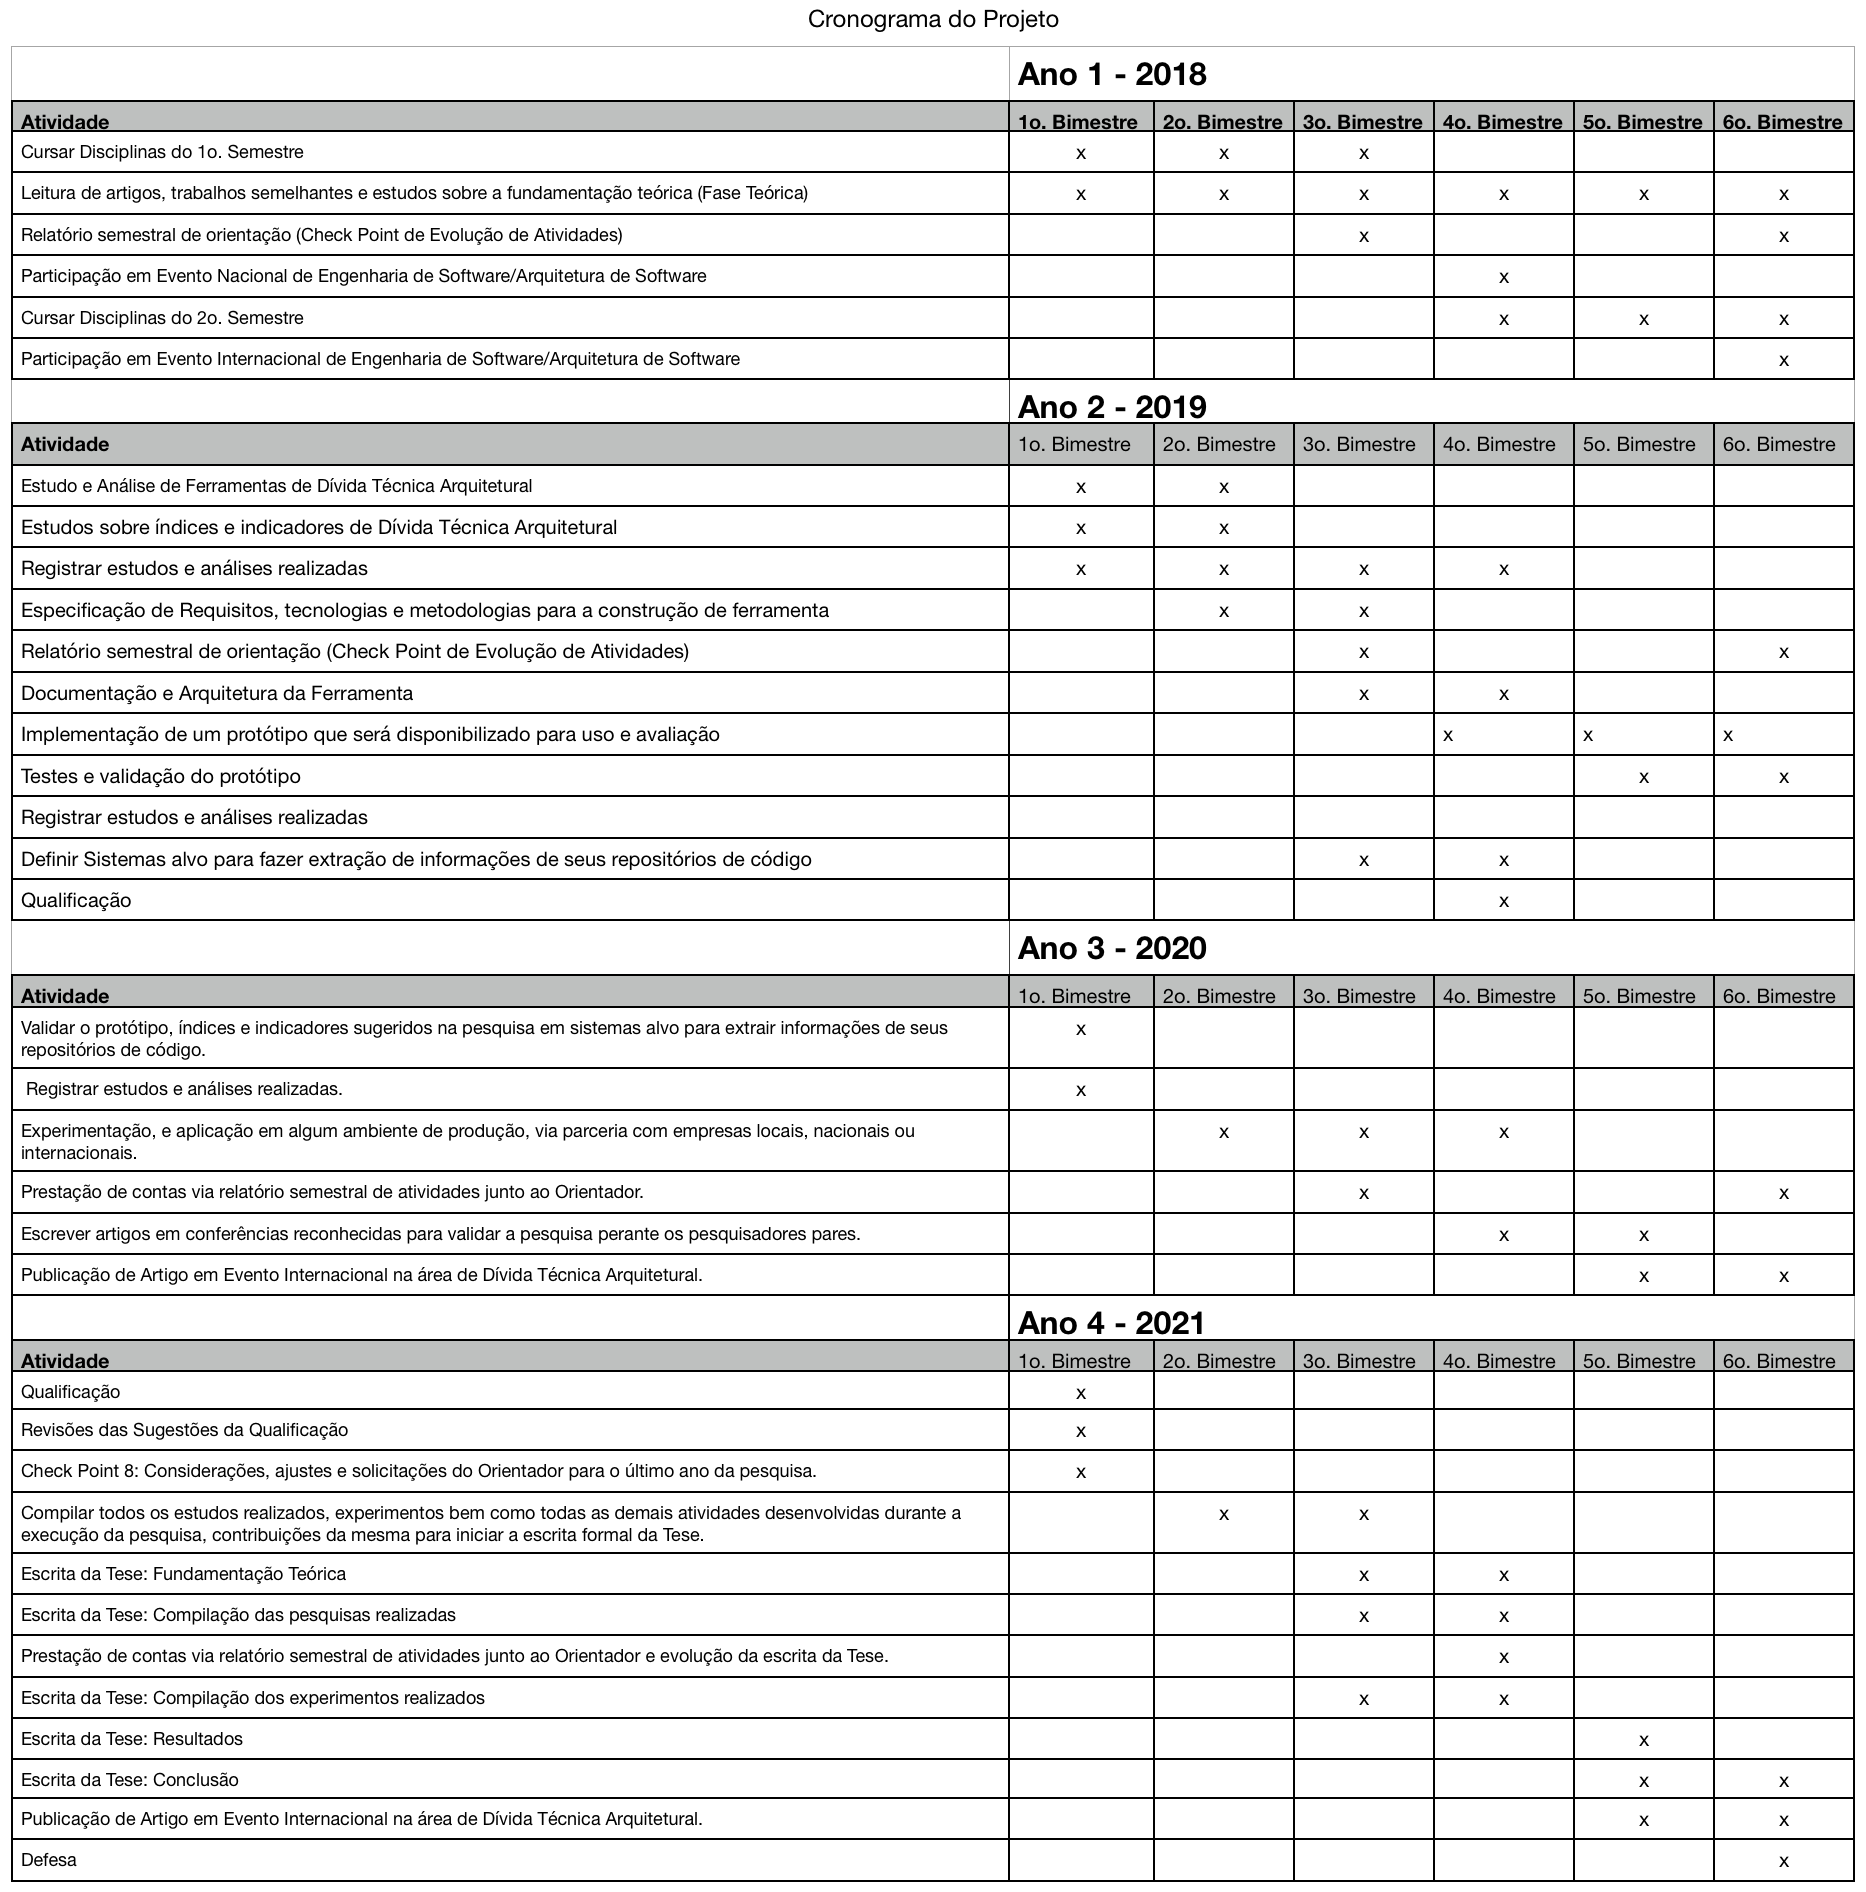
\includegraphics[scale=0.45]{cronograma.png}

Vale ressaltar que as atividades podem sofrer alterações de acordo
com as avaliações do orientador nos pontos de checagem da pesquisa.
\pagebreak{} 

% ----------------------------------------------------------
% Capitulo com exemplos de comandos inseridos de arquivo externo 
% ----------------------------------------------------------

\include{abntex2-modelo-include-comandos}

% ---
% Finaliza a parte no bookmark do PDF, para que se inicie o bookmark na raiz
% ---
\bookmarksetup{startatroot}% 
% ---

% ----------------------------------------------------------
% Referências bibliográficas
% ----------------------------------------------------------
\bibliography{Bibliografia-Pre-projeto-Doutorado}

\end{document}